%!TEX root = ../../main.tex

\documentclass[../../main.tex]{subfiles}

\begin{document}
	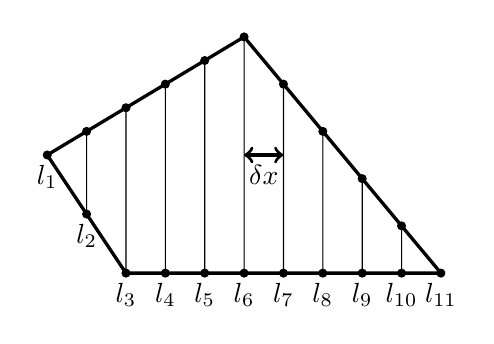
\begin{tikzpicture}[scale=1]

		\draw[very thick] (1,0)--(5,0)--(2.5,3)--(0,1.5)--(1,0);
		\draw[fill] (0,1.5) node [below] {$l_1$}circle [radius=0.05];
		\draw[fill, -] (0.5,0.75) node  [below]{$l_2$} circle [radius=0.05]--(0.5,1.8) node{} circle [radius=0.05];
		\draw[fill, -] (1.0,0.0) node [below]{$l_3$} circle [radius=0.05]--(1,2.1) node {} circle [radius=0.05];
		\draw[fill, -] (1.5,0.0) node [below]{$l_4$} circle [radius=0.05]--(1.5,2.4) node{} circle [radius=0.05];
		\draw[fill, -] (2.0,0.0) node [below]{$l_5$} circle [radius=0.05]--(2.0,2.7) node{} circle [radius=0.05];
		\draw[fill, -] (2.5,0.0) node [below]{$l_6$} circle [radius=0.05]--(2.5,3.0) node{} circle [radius=0.05];
		\draw[fill, -] (3.0,0.0) node [below]{$l_7$} circle [radius=0.05]--(3.0,2.4) node{} circle [radius=0.05];
		\draw[fill, -] (3.5,0.0) node [below]{$l_8$} circle [radius=0.05]--(3.5,1.8) node{} circle [radius=0.05];
		\draw[fill, -] (4.0,0.0) node [below]{$l_9$} circle [radius=0.05]--(4.0,1.2) node{} circle [radius=0.05];
		\draw[fill, -] (4.5,0.0) node [below]{$l_{10}$} circle [radius=0.05]--(4.5,0.6) node {} circle [radius=0.05];
		\draw[fill, -] (5.0,0.0) node [below]{$l_{11}$} circle [radius=0.05]--(5.0,0.0) node {} circle [radius=0.05];

		\draw[very thick, <->] (2.5,1.5)--(3,1.5);

		\node [below] at (2.75,1.5) {$\delta x$};

	\end{tikzpicture}
\end{document}